\documentclass[12pt,letterpaper]{article}
\usepackage[utf8]{inputenc}
\usepackage{amsmath}
\usepackage{amsfonts}
\usepackage{amssymb}
\usepackage{graphicx}

\usepackage[margin=1.1in]{geometry}


\begin{document}
\title{Progress Report}  \date{\vspace{-10ex}}

\maketitle

\par Using the ATLAS experiment at the Large Hadron Collider (LHC) a search for rare top quark decays in proton-proton collisions,  with center of mass energy $\sqrt{s}$ = 13 TeV is ongoing by Professor James Brau and graduate student Jason Barkeloo.  This search follows a similar search done at $\sqrt{s}$= 8 TeV which was able to set new limits on the branching ratio of the rare top quark flavor-changing neutral current (FCNC) decay modes where a top quark decays to an up-type quark (up or charm) and a photon.

\par Within the Standard Model (SM) of particle physics the top quark decays to a W boson and a bottom quark (t $\rightarrow$ bW) almost 100$\%$ of the time. A neutral current decay, in which the top quark decays to a neutral boson (photon, Z quark or Higgs boson) and an up-type quark (e.g. t $\rightarrow q\gamma$) is heavily suppressed through the GIM-Mechanism \cite{gim} as well being off-diagonal in the CKM-Matrix \cite{ckm}.  These FCNC processes can occur through higher-order loop processes.  However, these processes are significantly more rare: SM branching ratios for these FCNC decays of the top quark are of order $ 10^{-17}$ to $10^{-12}$ \cite{snowmass}, as seen in Figure \ref{fig:FCNCSummary}.  These ratios are significantly beyond both current and potential future experimental reach.  Many beyond the standard model theories exist which predict large enhancements to the top sector of the SM (e.g. various models of supersymmetry, Randall-Sundrum models, 2 Higgs Doublet models).  Observation of these FCNC decays would require a very large enhancement, eight to twelve orders of magnitude, to the SM Branching ratio and would be an absolute indication of new physics.  Current upper limits on the branching ratio BR(t $\rightarrow q\gamma$) from the CMS experiment at the LHC are BR($t \rightarrow c\gamma$) $< 1.7\text{x}10^{-3}$ and BR($t \rightarrow u\gamma$) $< 1.3\text{x} 10^{-4}$, with the full 8 TeV data set\cite{cms}.  

\par We are preforming a search for the FCNC in the $t\bar{t} \rightarrow bWq\gamma$ channel at ATLAS, using $\sqrt{s}$ = 13 TeV $pp$ collisions.  Specialized Monte Carlo simulation events for this process have been created after validation with the ATLAS collaboration's top quark group.  MadGraph was used to force the decays of the top quark to this specific final state.  These simulated events are reconstruced using a model of the ATLAS detector and have been created for all of the decay channels of the FCNC process for top-quark pair events including the top or antitop undergoing FCNC decay while the other goes through the SM typical decay.  The W boson decays are included as well and large signal samples have been produced for the leptonic mode (W $\rightarrow l \nu$) final state.  Working with the Monte Carlo production team to debug issues with the grid sites and Mad Graph samples were produced for each of the three Monte Carlo campaigns to correspond with different run parameters of Run 2 at the LHC.  A total of 660,000 events were simulated for each of the four signal final states mentioned.

\par There are many SM processes that can mirror the final state of our signal processes including $t\bar{t}$, W+jets, Z+jets, including processes that have an associated photon as well.  A cut based analysis is being executed to eliminate as much background as possible by optimizing the amount of signal in specific regions of phase space and look for an excess of events.  Validation regions orthogonal to the signal region have been produced to check Monte Carlo modeling of background samples.  These regions have minimal signal contamination but were created to have an enhanced amount of a specific background process.  We are using these orthogonal regions to ensure accuracy of our background modeling while our signal region is blinded.  After background studies have ensured a well modeled system we will move to unblind the study and search for any excesses in the signal region.  Any excess would imply some new physics otherwise a new branching ratio can be set which will help restrict current and future theoretical models.

\begin{figure}
\centering
 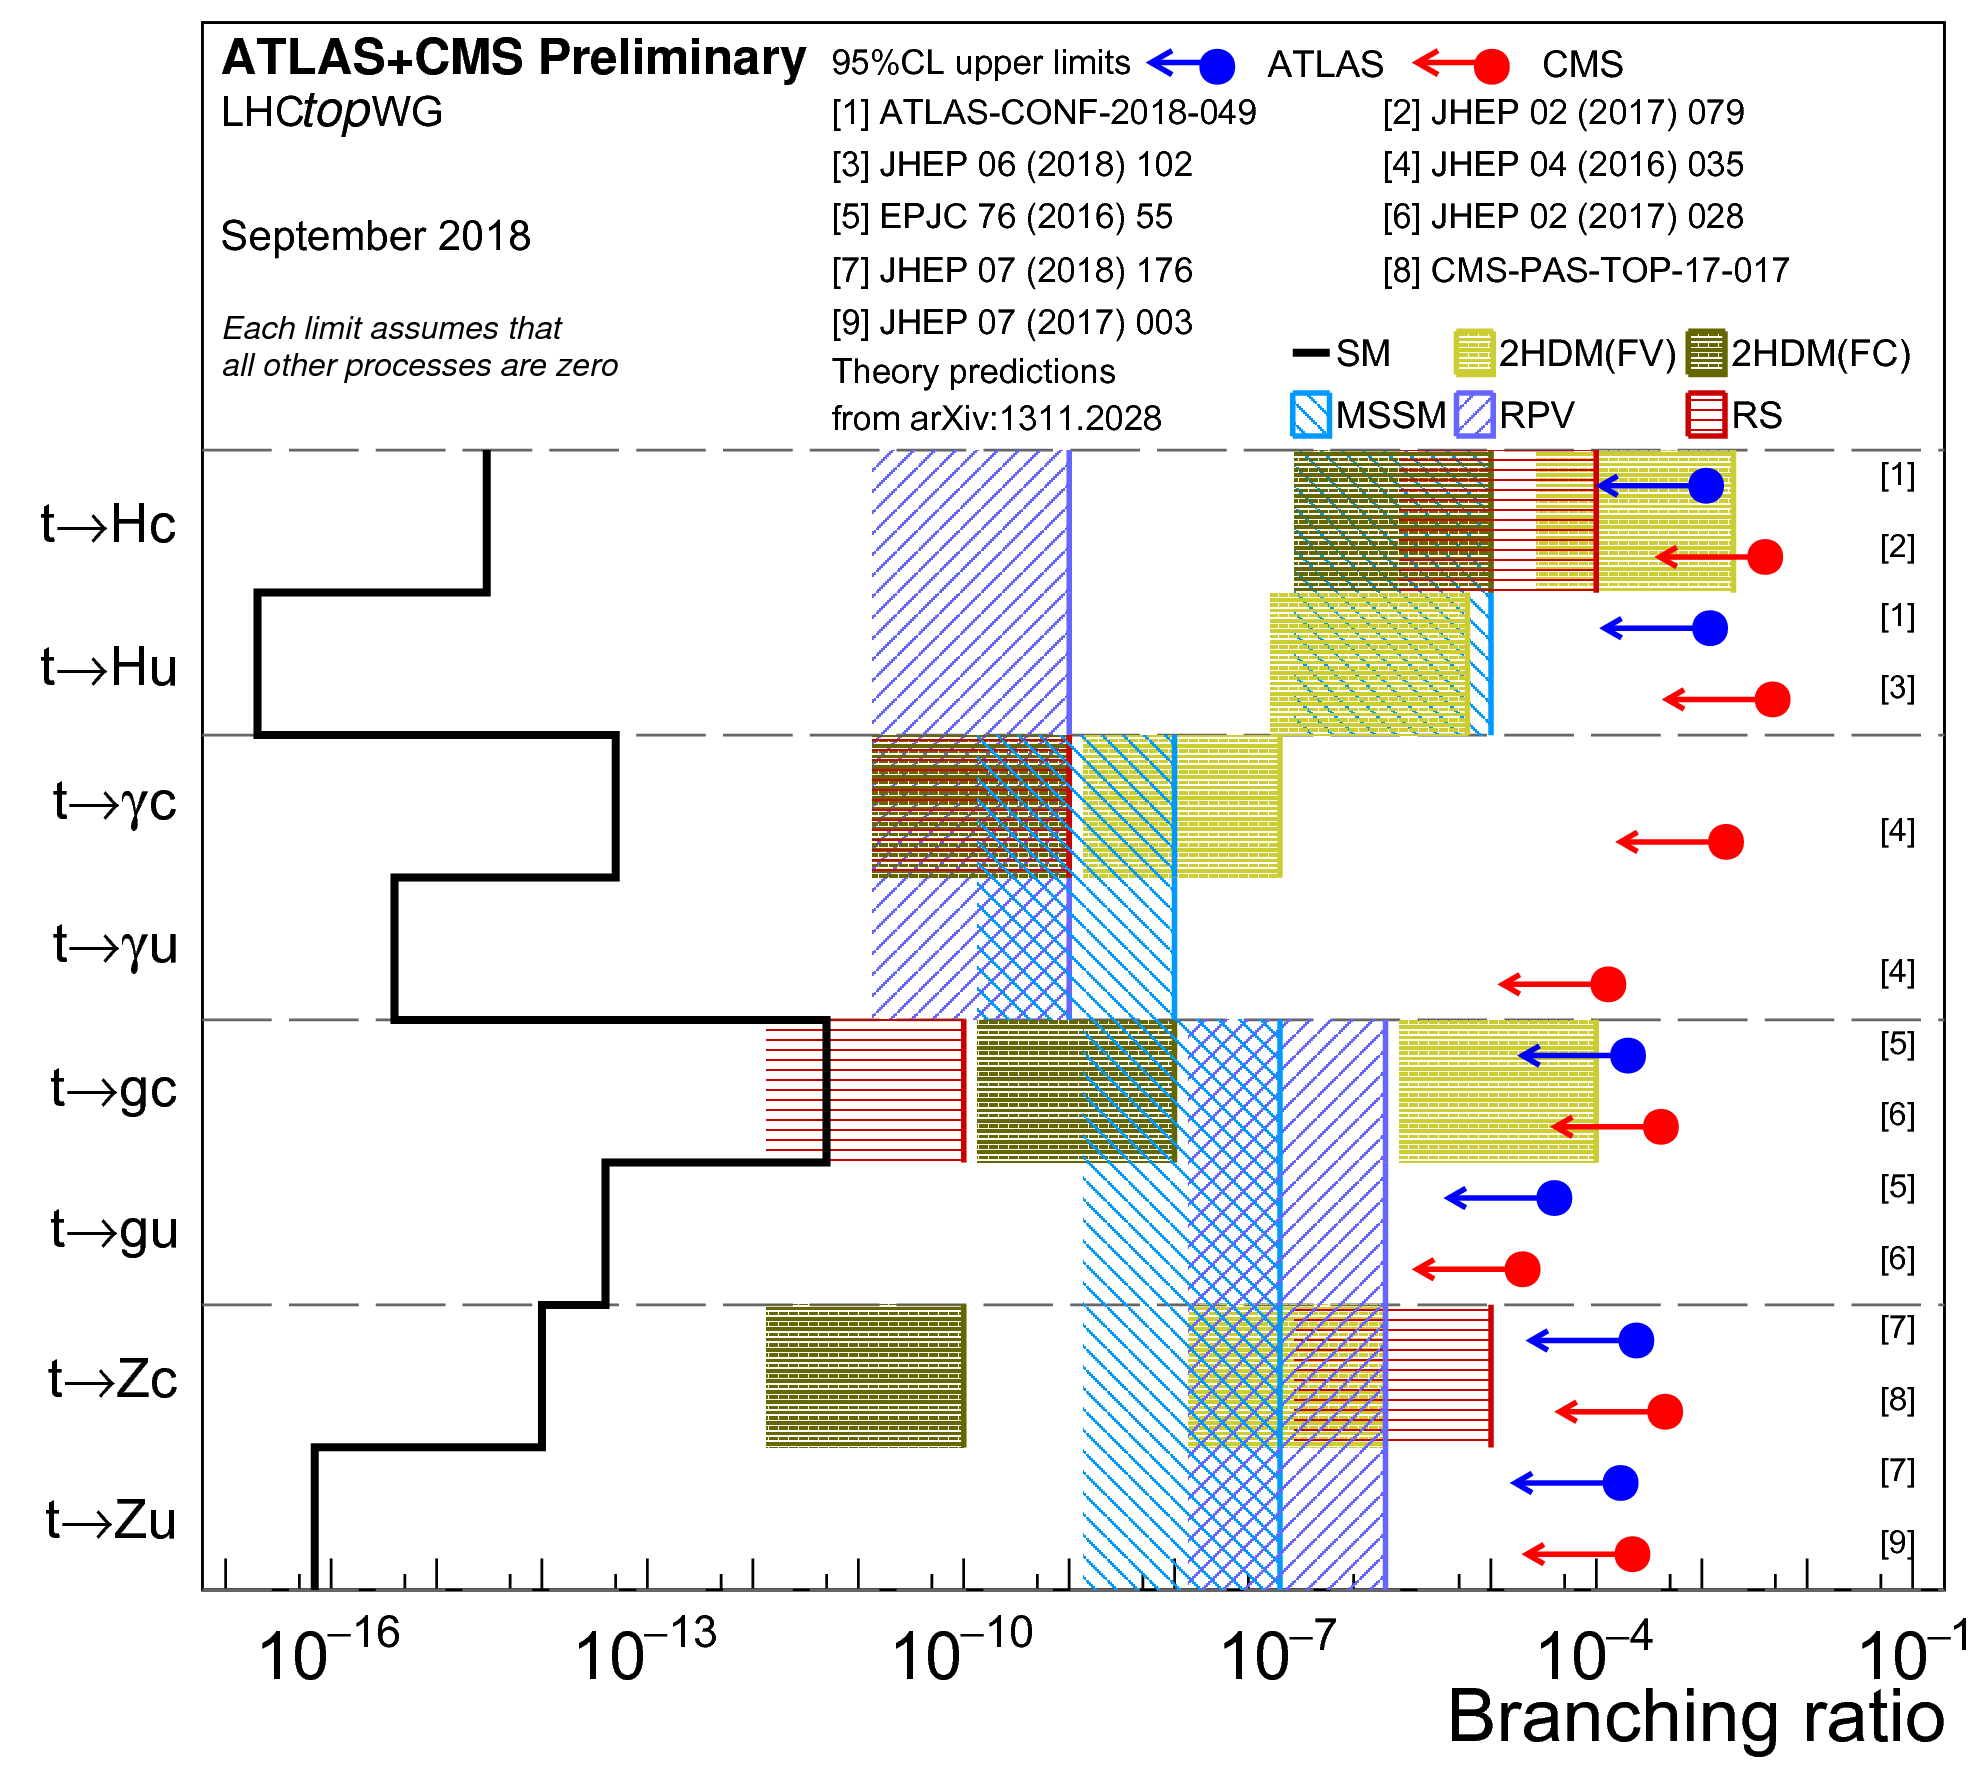
\includegraphics[width=0.5\textwidth]{FCNCSummary.png}
\caption{Summary plots of current 95\% confidence level ATLAS and CMS experimental limits compared to SM predictions and several new physics model predictions. \cite{TopWGPlots}}
\label{fig:FCNCSummary}
\end{figure}

\begin{thebibliography}{9}
\bibitem{gim} 
  S.~L.~Glashow, J.~Iliopoulos and L.~Maiani,
  %``Weak Interactions with Lepton-Hadron Symmetry,''
  Phys.\ Rev.\ D {\bf 2}, 1285 (1970).
  doi:10.1103/PhysRevD.2.1285
  %%CITATION = doi:10.1103/PhysRevD.2.1285;%%
  %5537 citations counted in INSPIRE as of 12 Dec 2017

\bibitem{ckm} 
  M.~Kobayashi and T.~Maskawa,
  %``CP Violation in the Renormalizable Theory of Weak Interaction,''
  Prog.\ Theor.\ Phys.\  {\bf 49}, 652 (1973).
  doi:10.1143/PTP.49.652
  %%CITATION = doi:10.1143/PTP.49.652;%%
  %9301 citations counted in INSPIRE as of 12 Dec 2017

\bibitem{snowmass} 
  K.~Agashe {\it et al.} [Top Quark Working Group],
  %``Working Group Report: Top Quark,''
  arXiv:1311.2028 [hep-ph].
  %%CITATION = ARXIV:1311.2028;%%
  %102 citations counted in INSPIRE as of 12 Dec 2017

\bibitem{cms}
  CMS Collaboration,
  ``Search for anomalous single top quark production in association with a photon in pp collisions at sqrt(s) = 8 TeV,''
  arXiv:1511.03951v2 [hep-ex].
  %%CITATION = ARXIV:1511.03951v2;%%
  %20 citations counted in INSPIRE as of 8 Sep 2016

\bibitem{TopWGPlots}
LHCtopWG, LHC Top Working Group Summary Plots
\\\texttt{https://twiki.cern.ch/twiki/bin/view/LHCPhysics/LHCTopWGSummaryPlots}
\end{thebibliography}
\end{document}